
\section{The \app Framework Overview}

\begin{figure*}[tbp] \centering
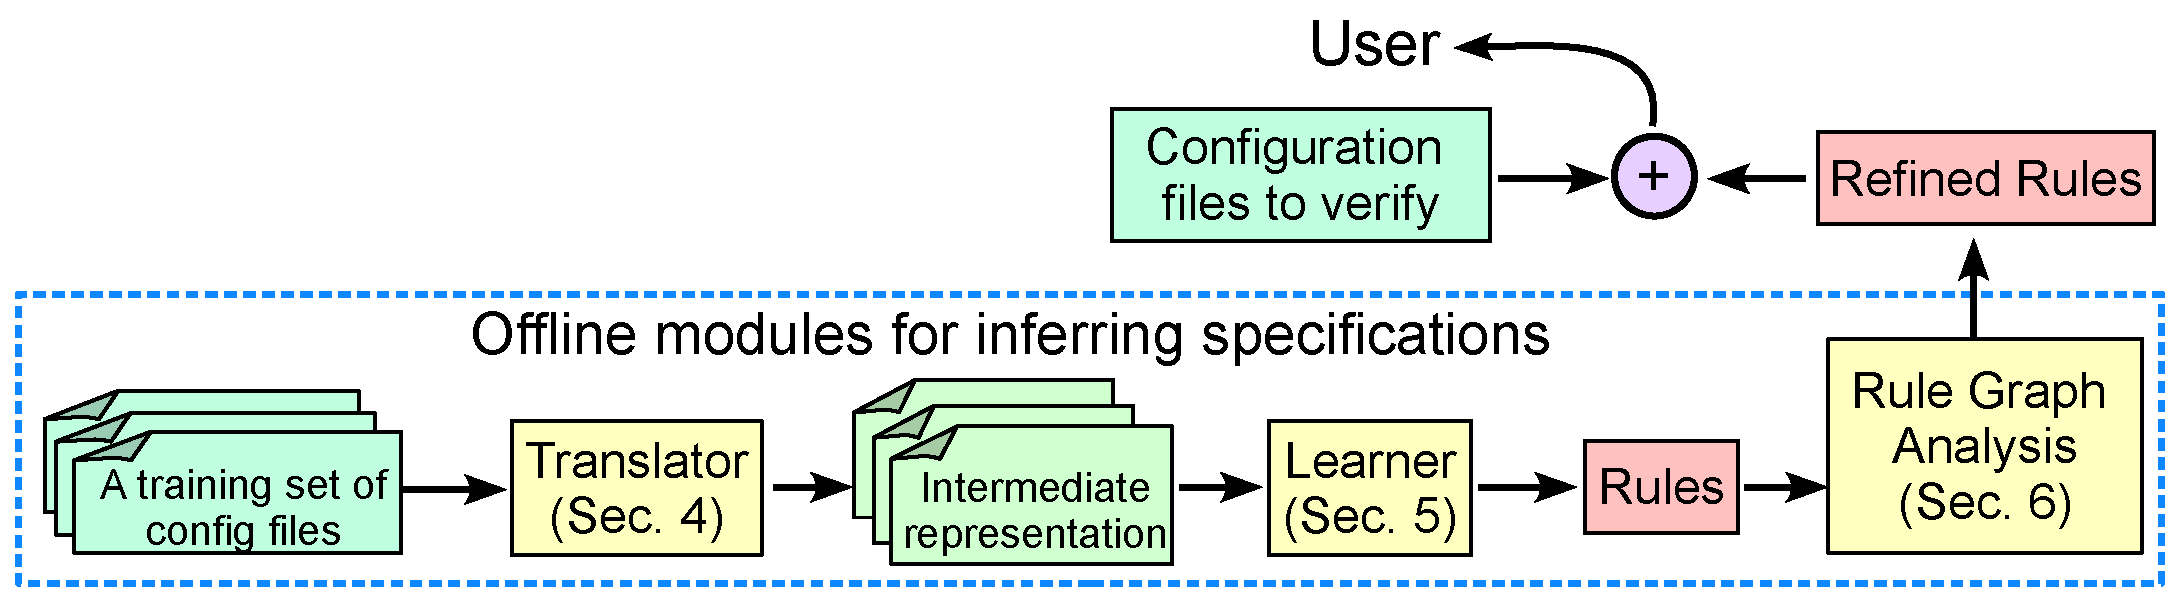
\includegraphics[width=0.88\textwidth]{figs/overview}
\caption{\app's workflow. The green components represent configuration 
  files, including both sample configuration datasets and users' input
  configuration files to verify.
  The blue dashed box is \app. 
  The yellow components are key modules of \app.
  The purple circle is a checker for checking whether the target
  configuration file violates any rule.}
\label{fig-overview}
\end{figure*}

We propose \app, an automatic verification framework for 
software configuration files.
In particular, \app can detect many sophisticated configuration errors, 
including ordering errors, missing entry errors,
type errors and integer correlation errors. 
As depicted in Figure~\ref{fig-overview}, 
a typical \app verification workflow has three steps:
translation, learning, and rule refinement. In this section, we briefly
describe how each step works.

\para{Initial phase.}
We start with the assumption 
that we are given a number of (not necessarily correct) 
configuration files, called {\em sample dataset}, 
belonging to the same system, such as MySQL or Apache. 
These files, therefore, follow similar patterns.
%In the following steps,
%we will exploit in a collection of learning algorithms 
%to build rules that describe a language model for the files.

\para{Translator.}
The translator module first parses the input sample 
dataset of configuration files, and then transforms them into 
a more structured and typed intermediate representation.
When we infer the types of entries in a configuration file, 
the type of an entry cannot always be fully determined from 
a single value, since it is very hard to understand
the purposes of key-value entries in modern
software configuration files~\cite{xu15hey}.
We address this problem 
by introducing {\em probabilistic types}.
Rather than giving a variable a single type, 
we assign several types over a probability distribution. 
We can later use these more structured files
as a training set to learn the rules. 

\para{Learning.}
The input of the learner is a set of files that have been translated
into well-structured intermediate representations. 
The learner employs a learning algorithm named {\em rule association 
algorithm} to generate various rules,
potentially used to handle different types of configuration errors,
including ordering errors, missing entry errors,
type errors and integer correlation errors.
These rules are the outputs of the learner, 
and will be used to detect errors later.
Because the translator gives the learner probabilistically typed entries,
the learner is also responsible for determining a type for each entry.

\para{Rule refinement.}
The checker is used to detect rule violations in the configuration
files of interest. The inputs of the checker are the learned rules 
and the target configuration file to verify.
It generates a report (as shown in $\S$\ref{sec-motiv}) about 
whether it finds any error, \eg, rule violations 
or some suspicious values (\eg, singular value anomaly).
As shown in Figure~\ref{fig-overview},
there are two sub-modules in the checker. They are responsible for
checking rule violations and suspicious values, respectively.
In our experience, we found learned rules could be significantly reused
to check different configuration files, thus improving our usability.  
